%%%%%%%%%%%%%%%%%%%%%%%%%%%%%%%%%%%%%%%%%%%%%%%%%%%%%%%%%%%%%%%%%%%%%%%%
%
% hierarchical Inference in Weak Lensing: Inferring Pr(e)
%
%%%%%%%%%%%%%%%%%%%%%%%%%%%%%%%%%%%%%%%%%%%%%%%%%%%%%%%%%%%%%%%%%%%%%%%%

\documentclass[useAMS,usenatbib]{mn2e}
%% letterpaper
%% a4paper

% \voffset=-0.8in

% Packages:
% \input psfig.sty
\usepackage{xspace}
\usepackage{graphicx}

% Macros:
% JOURNALS
\newcommand {\apj} {ApJ}
\newcommand {\apjl} {ApJL}
\newcommand {\apjs} {ApJS}
\newcommand {\mnras} {MNRAS}
\newcommand {\apss} {Ap \& SS}
\newcommand {\aap} {A\&A}
\newcommand {\aj} {AJ}
\newcommand {\prd} {Phys. Rev. D}
\newcommand {\nat} {Nature}
\newcommand {\araa} {ARA\&A}
\newcommand {\jgr} {J. Geophys. Res.}
\newcommand {\pasp} {PASP}

% MISC
\newcommand {\etal} {et~al.~}
\def \spose#1{\hbox  to 0pt{#1\hss}}  
\newcommand {\lta} {\mathrel{\spose{\lower 3pt\hbox{$\sim$}}\raise  2.0pt\hbox{$<$}}}
\newcommand {\gta} {\mathrel{\spose{\lower  3pt\hbox{$\sim$}}\raise 2.0pt\hbox{$>$}}}
\def \ion#1#2{#1{\footnotesize{#2}}\relax}
\newcommand {\ha}  {\ifmmode H\alpha \else H$\alpha $ \fi} 
\newcommand {\hi} {\ion{H}{I} } 

\def\Sref#1{Section~\ref{#1}\xspace}
\def\Fref#1{Figure~\ref{#1}\xspace}
\def\Tref#1{Table~\ref{#1}\xspace}
\def\Eref#1{Equation~\ref{#1}\xspace}
\def\Eqref#1{Eq.~(\ref{#1})\xspace}

% UNITS
\newcommand {\kms} {\ifmmode  \,\rm km\,s^{-1} \else $\,\rm km\,s^{-1}  $ \fi }
\newcommand {\kpc} {\ifmmode  {\rm kpc}  \else ${\rm  kpc}$ \fi  }  
\newcommand {\pc} {\ifmmode  {\rm pc}  \else ${\rm pc}$ \fi  }  
\newcommand {\Msun} {\ifmmode {\rm M_{\odot}} \else ${\rm M_{\odot}}$ \fi} 
\newcommand {\Zsun} {\ifmmode {\rm Z_{\odot}} \else ${\rm Z_{\odot}}$ \fi} 
\newcommand {\yr} {\ifmmode yr^{-1} \else $yr^{-1}$ \fi} 
\newcommand {\hMsun} {\ifmmode h^{-1}\,\rm M_{\odot} \else $h^{-1}\,\rm M_{\odot}$ \fi}

% COSMOLOGY
%\newcommand {\LCDM} {\ifmmode \Lambda{\rm CDM} \else $\Lambda{\rm CDM}$ \fi}

% LENSING
\def\zd{z_{\rm d}}
\def\zs{z_{\rm s}}
\def\zspdf{z_{\rm s,pdf}\;}
\def\Dd{D_{\rm d}}
\def\Ds{D_{\rm s}}
\def\Dds{D_{\rm ds}}
\def\Sigmacrit{\Sigma_{\rm crit}}

% SOFTWARE/HARDWARE
\def\SExtractor{{\sc SExtractor}\xspace}
\def\hst{{\it HST}\xspace}
\def\acs{\hst/ACS\xspace}
\def\galfit{{\sc galfit}\xspace}
\def\idl{{\sc idl}\xspace}
\def\python{{\sc python}\xspace}

% PROBABILITY THEORY
\def\pr{{\rm Pr}}
\def\data{{\mathbf{d}}}
\def\datap{{\mathbf{d}^{\rm p}}}
\def\datai{d_i}
\def\datapi{d^{\rm p}_i}
\def\pars{\boldsymbol{\theta}}

% COMMENTING
\usepackage[usenames]{color}
\newcommand{\phil}[1]{\textcolor{blue}{\bf #1}}
\newcommand{\hogg}[1]{\textcolor{green}{\bf #1}}
\newcommand{\flag}[2]{\textcolor{red}{\it\bf #1: #2}}

\def\oxford{Department of Physics, University of Oxford, Keble Road, Oxford, OX1 3RH, UK}
\def\nyu{Center for Cosmology and Particle Physics, New York University, NY, USA}



%%%%%%%%%%%%%%%%%%%%%%%%%%%%%%%%%%%%%%%%%%%%%%%%%%%%%%%%%%%%%%%%%%%%%%%%

\title[Hierarchical Inference in Weak Lensing]
{Hierarchical Inference of the Intrinsic Ellipticity
Distribution of Galaxies during Weak Lensing Analysis}
    
\author[Tang et al]{%
  Yike~Tang$^{1}$,
  David W. Hogg,$^{1}$
  Philip~J.~Marshall$^{2}$
  \medskip\\
  $^1$\nyu\\
  $^2$\oxford
}

%%%%%%%%%%%%%%%%%%%%%%%%%%%%%%%%%%%%%%%%%%%%%%%%%%%%%%%%%%%%%%%%%%%%%%%%

\begin{document}
             
\date{to be submitted to MNRAS}
             
\pagerange{\pageref{firstpage}--\pageref{lastpage}}\pubyear{2010}

\maketitle           

\label{firstpage}

%%%%%%%%%%%%%%%%%%%%%%%%%%%%%%%%%%%%%%%%%%%%%%%%%%%%%%%%%%%%%%%%%%%%%%%%
% in this abstract, below, check the use of -, --, and ---.  Understand?

\begin{abstract}
Weak-lensing projects---to measure galaxy--galaxy lensing or the shear--shear
correlation function---often make use of estimators that involve simple or weighted
means of measured galaxy ellipticities.  Here we propose moving to a probabilistic inference
framework for weak-lensing projects, in which the both the distribution of unlensed
(intrinsic) galaxy ellipticities and the distribution of ellipticity measurement noise contributions
are both treated as priors.  We perform hierarchical inference to \emph{infer} the
unlensed ellipticity distribution simultaneously with the shear map.  The best
shear-field estimates, in this context, become the \emph{marginalized}-likelihood functions, in which uncertainty about the
inferred unlensed distribution has been marginalized out.  We show that our proposed
estimates do not give a significant bias when averaged by statistical weight and perform better than simple mean-ellipticity estimators both in terms of variance.
We also show that as the number of observed galaxies becomes
large, the performance of our proposed estimators approaches the performance of a
magical maximum-likelihood estimator that could be constructed if the true unlensed
ellipticity distribution were known \textit{a priori}.  Importantly, this work only
considers the \emph{catalog-level} problem of how to combine galaxy ellipticity
measurements; it does not consider the problem of making those measurements in the
first place.  In the end we argue that weak lensing projects ought to move beyond
point estimates and instead propagate full likelihood-function information about
the shear field forward into scientific analyses. Only this could properly
propagate uncertainty without introducing additional catalog-generated variance.
\end{abstract}

% Full list of options at http://www.journals.uchicago.edu/ApJ/instruct.key.html

\begin{keywords}
  gravitational lensing
\end{keywords}

\setcounter{footnote}{1}

%%%%%%%%%%%%%%%%%%%%%%%%%%%%%%%%%%%%%%%%%%%%%%%%%%%%%%%%%%%%%%%%%%%%%%%%
%%  SECTION 1: INTRODUCTION
%%%%%%%%%%%%%%%%%%%%%%%%%%%%%%%%%%%%%%%%%%%%%%%%%%%%%%%%%%%%%%%%%%%%%%%%



\section{Introduction}

\label{sec:intro}

\flag{Yike}{Plan the sections of your paper, and write very brief
notes on what you want to say in each of them. You will find it helpful
to divide them into sub-sections, and even paragraphs. You may also
want to put in placeholder figures and tables; if you do, make sure
to write the captions of them. The itemized conclusions should be
partial answers to a corresponding list of questions in the introduction.
You can write these now, as incomplete statements: when you know what
your findings are, you can complete them.}

% WL as cosmological and astrophysical probe. 


% Information is scarce. 
% Expensive, high precision future. Motivation.


% This paper: toy problem, exploring one aspect of analysis.


% History of shear estimation, and treatment of Pr(e).


Weak gravitational lensing has the potential to be the most powerful
tool to explore the dark universe. One application of weak gravitational lensing is
that it can be used to measure the mass profile of single galaxy, galaxy
groups, clusters and the large scales. Cosmic shear is the mild distortion
of distant galaxy images due to the bending of light by intervening
matter. It provides one of the most promising methods for constraining
the nature of dark energy (Albrecht et al. 2006; Peacock\&Schneider
2006). While in galaxy--galaxy weaklensing, tangential shear distortions
of background galaxies around foreground galaxies allows direct measurement
of the galaxy-DM correlation.

The distortion of galaxy image caused by weak lensing effect is typically only a few percent.
It's usually more than 10 times smaller than galaxies' intrinsic ellipticity. It's also smaller than the distortion caused
by the PSF effect which is usually around 0.05 level. The main source of uncertainty of shear measurements is the intrinsic shape noise
. Since the unlensed galaxy shape can not be observed directly, the information
we have about the intrinsic ellipticity is scarce. One natural assumption about the intrinsic shape distribution is that 
it should be isotropic. With this assumption, an estimator can be made by simply averaging galaxies' complex
ellipticity. However by doing this we are not be able to utilize the
information about how the ellipticity are distributed. The mean ellipticity
point estimator can't use another reasonable assumption about the intrinsic shape distribution - galaxies in different sky patches should have
the same shape distibution - which is a natural result of the homogeneous Universe.

A typical procedure of weak lensing analysis  includes galaxy shape measurements from images
, shear inference and mass profile reconstruction. The galaxy shape measurement is usually the
first step of weak lensing analysis, since it's a direct observable of shear effect. However
in this paper we only concern about how to infer shear from galaxy
ellipticity in a novel hierarchical way. Therefore we set up a simple toy model in which we have the observed ellipticity as
data, and the only shape measurement error we consider is a Gaussian noise
added on the lensed galaxy ellipticity. We also suppose there is a uniform shear
acting on all the galaxies in one sky patch.

Our approach is to use an exceedingly flexible model for intrinsic
shape distribution, and assumes all the galaxies in different patches
abey such a distribution. Then we can calculate the joint likelihood
of shape distribution parameters and shear in different sky patches. Using
 Gibbs MCMC sampler we are able to sample the joint posterior distribution
in an efficient way. After marginalizing the shape parameters, we can obtain
the posterior distribution of shear, which we are interested in. This
approach allows us to use the information maximumly without introducing
in any wrong assumption on the intrinsic shape distribution.

In galaxy--galaxy lensing, since the distortion is so weak, what people
usually do is to stack many lensing signals together. Then the mean
shear map and mean mass profile of single galaxy or galaxy
cluster can be inferred from this stacked lensing signal. However with the Hierarchical Bayesian method we can avoid this brute averaging
of lensing signal. Instead, we can get the posterior distribution of mass profile for
each lensing system, even though it may have very large uncertainty. Then we
can calculate their statistical properties like galaxy-mass correlation
function via this posterior distribution.

This paper is orgnized as following: In section 2 we introduce the
weak lensing formulas and the likelihood functions. Then we describe
two flexible models for the intrinsic shape distribution. Section 3 details
the results of simulations including tests for biases and accuracy. In Section 4, we
derive some general conclusions and outline suggestions for future
development.

%%%%%%%%%%%%%%%%%%%%%%%%%%%%%%%%%%%%%%%%%%%%%%%%%%%%%%%%%%%%%%%%%%%%%%%%
%%  SECTION N: XXX
%%%%%%%%%%%%%%%%%%%%%%%%%%%%%%%%%%%%%%%%%%%%%%%%%%%%%%%%%%%%%%%%%%%%%%%%



\section{Method}

\label{sec:XXX}


\subsection{Likelihood Functions}

We assume the lensed galaxy ellipticity $\epsilon_{\ell}$ is related
to the intrinsic galaxy ellipticity $\epsilon_{0}$ in the weak lensing
regime via 
\begin{equation}
\epsilon_{\ell}=\frac{\epsilon_{0}+g}{1+g^{*}\epsilon_{0}}
\end{equation}


and it's inverse formula 
\begin{equation}
\epsilon_{0}=\frac{\epsilon_{\ell}-g}{1-g^{*}\epsilon_{\ell}}
\end{equation}
from Schramm \& Kayser (1995), Seitz \& Schneider (1997), where $\epsilon$
is represented as a complex variable. It is defined in terms of the major and minor axes and orientation a, b, $\phi$,
respectively, as
\begin{equation}
\epsilon=\frac{a-b}{a+b}e^{2i\phi}
\end{equation}
$g$, $g^{*}$ are the reduced shear and its complex conjugate, respectively. In weak lensing region we have 
\begin{equation}
g=\frac{\gamma}{1-k}\approx\gamma
\end{equation}
$\gamma$ is the shear. This is the assumption we use through out
the paper.
Due to the isotropicity of the Universe, for the unlensed ellipticity $\epsilon_{0}$ 
we expect $\phi$ has a uniform distribution
from 0 to $\pi$. Then we can expect 
\begin{equation}
<\epsilon_{\ell}>=g
\end{equation}
Therefore $<\epsilon_{\ell}>$ can be adopted as an estimator of g.

However in our hierarchical Bayesian approach we are able to obtain
the posterior distribution of reduced shear, based on the assumption that $\phi$ has
a uniform distribution and galaxies in different sky patches have
the same intrinsic shape distribution.

Suppose we know the intrnsic ellipticity distribution $P(\epsilon_{0}|\vec{\alpha})$
based on some parasmeters $\vec{\alpha}$. Then we can write down the joint likelihood
of reduced shear $g$ and shape parameters $\vec{\alpha}$:

\begin{equation}
p(\epsilon_{\ell}|\vec{g},\alpha)=p(\epsilon_{0}(\vec{g})|\alpha)\,|\frac{\partial\epsilon_{0}}{\partial\epsilon_{\ell}}|
\end{equation}



Note that both $\epsilon_{0}$ and $\epsilon_{\ell}$ are complex numbers. So
$|\frac{\partial\epsilon_{0}}{\partial\epsilon_{\ell}}|$ is the Jacobian
determinant term, which is calculated numerically from formula
(5).

For a realistic unperfect galaxy shape measurement, there will be measurement errors on $\epsilon_{ob}$. Then we will have 
\begin{equation}
p(\epsilon_{ob}|\vec{g},\alpha)=\int f(\epsilon_{ob}|\epsilon_{\ell})\, p(\epsilon_{\ell}|\vec{g},\alpha)\,d\epsilon_{\ell}
\end{equation}
Here the prior distribtuion we use for $\vec{g}$ is a 2D flat distribution
in the region $|\vec{g}|<1$. Therefore $p(\vec{g)}=1$ if $|\vec{g}|<1$
and $p(\vec{g})=0$ if $|\vec{g}|>1$.

The prior of $\alpha$ some how depends on the model we choose for
intrinsic ellipticity distribution. When we use the step function
model for P($\epsilon_{0}$), which we'll describe latter, we find that
we need to use a prior regulazier on $\alpha$. 
\begin{equation}
p(\vec{\alpha}|\xi)=exp(-\xi\sum(\alpha_{i}-\alpha_{i-1})^{2})
\end{equation}

Given the likehood functions and priors we can also calculate the marginalized likelihood function. 
\begin{equation}
p(\epsilon_{\ell}|\vec{g})=\int p(\epsilon_{\ell}|\vec{g},\vec{\alpha})\,p(\vec{\alpha}|\vec{g})\,d\vec{\alpha}
\end{equation}

Since $p(\alpha)$ does not explicitly depend on $\vec{g}$. $p(\alpha|\vec{g})$ is
just the prior distribution $p(\vec{\alpha}|\xi)$. Therefore, we have
marginalized likehood 
\begin{equation}
p(\epsilon_{\ell}|\vec{g})=\int p(\epsilon_{\ell}|\vec{g},\vec{\alpha})\, p(\vec{\alpha}|\xi)\,d\vec{\alpha}
\end{equation}
Given that marginalized likelihood function, in principle we could optimize it and give out a max-likelihood estimator for $g$
in different patches simultaneously.

One thing to note is that the likelihood of $g$ in one patch only explicitly depends
on the shape parameters but not dependent to reduced shear in other patches. Therefore, the
marginalized likelihood of shape parameters is :

\begin{equation}
\ell(\alpha|data)=\prod_{i}\ell_{i}(\alpha|data_{i})
\end{equation}


$\ell_{i}(\alpha|data_{i})$ is the marginalized likelihood function
calculated with data in the ith patch. From this formula we can see
how better inference of $\vec{\alpha}$ will be obtained if we infer numerous
sky patches simultaneously. With better knowledge on $\vec{\alpha}$ we
will in turn have better estimates on the reduced shear $g$.


\subsection{Model for Intrinsic Shape Distribution}

The correctness of posterior distribution of $g$ depends on the intrinsic
ellipticity distribution P($\epsilon_{0}|\alpha$). Due to the limitation
of human's knowledge we will not be able to give an analytical form for
$P(\epsilon_{0}|\alpha)$. Therefore we propose an exceedingly flexible
model for $P(\epsilon_{0}|\alpha)$, which does not require further
assumption on $P(\epsilon_{0}|\alpha)$.

We divide the 2-D space r $\in$(0,1) into N bins. The probability
of each bin is $p_{i}=e^{\alpha_{i}}$. $\overrightarrow{\alpha}$
is a N dimension parameter to be inferred, simultaneously with $g$.

From practice we find that a prior smooth regularizer on $\vec{\alpha}$
is needed to obtain a good estimation on $g$ and $\vec{\alpha}$.

The prior distribution we used on $\vec{\alpha}$ is : 
\begin{equation}
p(\vec{\alpha}|\xi)=exp(-\xi\sum(\alpha_{i}-\alpha_{i-1})^{2})
\end{equation}

Here $\xi$ is a prefactor need to be tuned.
Meanwhile, in order to show the correctness of our method, we also
set up a simulation in which we know that the true $P(|\epsilon_{0}||\alpha)$
is a Beta distribution, and thus $\alpha$ is the 2-D parameter (p,q)
of the Beta distribution. We will show the posterior samples using
both of these two methods in next section. Note that for either model
we assume P($\epsilon_{0}$) is isotropic.

\subsection{Gibbs Sampler}

While making the posterior samples $p(\vec{g},\alpha|Data)$ we choose to
use the classical Gibbs sampler.

In Gibbs sampling, variables $x_{j}$ are sampled from the conditional
probability distribution: $p(x_{j}^{(i)}|x_{1}^{(i)},....,x_{j-1}^{(i)},x_{j+1}^{(i-1)}...,x_{n}^{(i-1)})$

The conditional probability distribution of one variable given all the other variables are proportional to their joint probability distribution

\begin{equation}
p(x_{j}|x_{1},....,x_{j-1},x_{j+1}...,x_{n})\propto p(x_{1},.....,x_{n})
\end{equation}


One thing to note is that the conditional probability of $g$ in one patch only explicitly depends on $\alpha$, but not g in other patches. Therefore
with $\vec{\alpha}$ fixed, the posterior distributions of reduced shear in different patches are independent from each other. 
\begin{equation}
p(\vec{g}_{1}....\vec{g}_{n}|\vec{\alpha},Data)=p(\vec{g}_{1}|\vec{\alpha},Data_{1})....p(\vec{g}_{n}|\vec{\alpha},Data_{n})
\end{equation}
Therefore sampling reduced shear g from the conditional probability distribution can be reduced to a 2D sampling problem, which can be done very quickly.
In the Gibbs sampler, first we make a sample of $p(\vec{\alpha}|\vec{g},Data)$ with Metropolis-Hasting sampler. The we make samples of $g$ in different patches
independently according to formula (14).
The total time needed to sample $g$ and $\alpha$ of 64 sky patches with 8 galaxies in each patch is 
approximitly 25s on a 2 GHz CPU.


\subsection{Simulations}

The procedure of our simulation is as following. First we generate N$\times$NP
unlensed galaxies' elliprticity from the ``true'' $P(\epsilon_{0})$, and
asign them into NP patches evenly. So each patch has N galaxies. Then
we generate NP true reduced shears, and asign them to each patch, and
then shear the unlensed galaxies using formula (4).

Finally we can add noise on $\epsilon_{\ell}$ to get the
observed ellipticity $\epsilon_{ob}$. For simplicity we've only considered
the situation where P($\epsilon_{ob}|\epsilon_{\ell})$ is a 2D Gaussian.

Use Gibbs sampler and $P(\epsilon_{0}|\alpha)$ mentioned previously, we
are to sample the posterior distribution of g and $\alpha$ simultaneously
and effectively.

%%%%%%%%%%%%%%%%%%%%%%%%%%%%%%%%%%%%%%%%%%%%%%%%%%%%%%%%%%%%%%%%%%%%%%%%
%%  SECTION N: XXX
%%%%%%%%%%%%%%%%%%%%%%%%%%%%%%%%%%%%%%%%%%%%%%%%%%%%%%%%%%%%%%%%%%%%%%%%



\section{Result}

\label{sec:XXX}


\subsection{Posterior Samples}
The probability distribution can be visualised by plotting points at each sample
position. An example in the x, y plane is shown for the posterior distribution of
$g$ in 64 sky patches in Figure 1. There are 8 galaxies in each patch in the simulation.
The number density of samples is proportional to the probability density. The figure shows that the two parameters of $\vec{g}$
do not have strong correlation, since the shape of smaples is close to a circle.
We also shows the histogram of g1 in a single sky patch in Figure 2. Not surprisingly it is close to a Gaussian distribution.
If the probability distribution of parameters are perfect Gaussian, the most probable estimates and uncertainty 
is just the mean and standard deviation of the Gaussian distribution. However, in pratical, we find that the distribution 
of reduced shear $\vec{g}$ will  get closer to Gaussian, when larger number of galaxies in one patch  is used. When the number of galaxies in 
one patch is equal to or larger than 8, we found it's eligible to make such an approximation that to use sample mean and standard 
deviation as the most probable estimates and uncertainty. We'll justify this approximation with a bias test in the following
sub section. 

\begin{figure}
\end{figure}
\begin{figure}
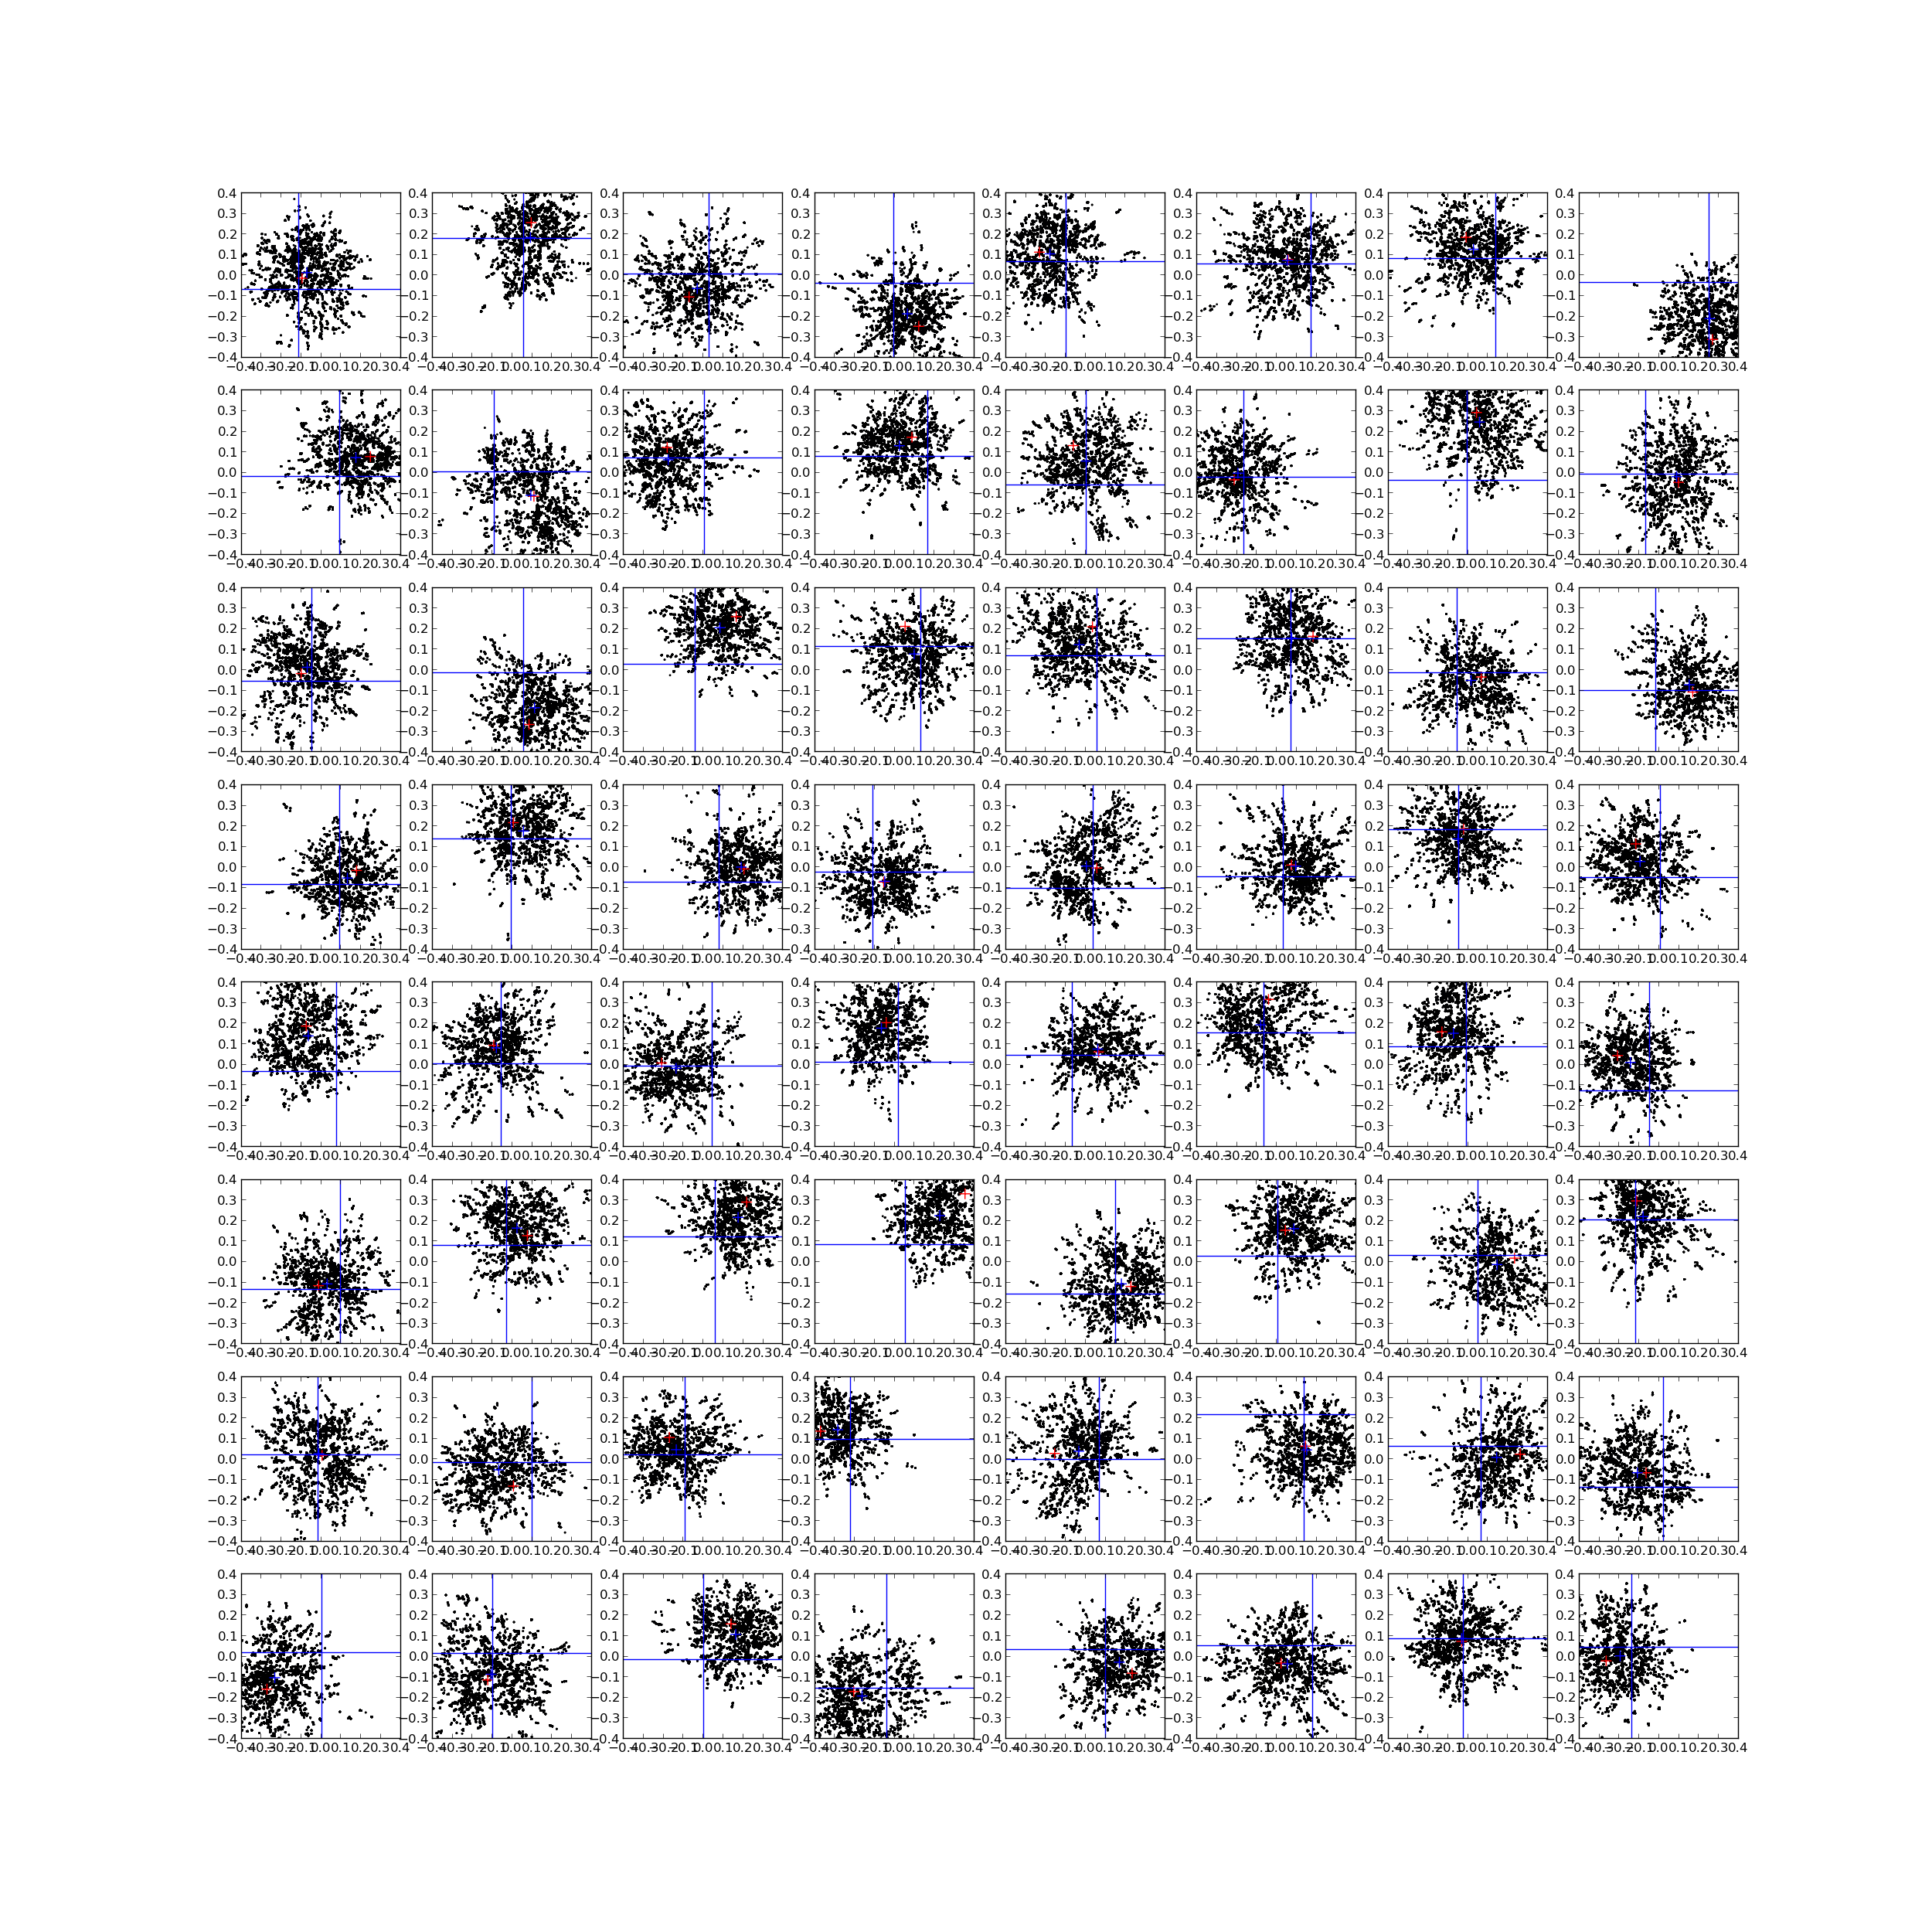
\includegraphics[scale=0.15]{fig/test10}

\caption{The figure shows the posterior samples of reduced shear g
in all the 64 patches. The two blues lines indicate the poisition of
true(input) $g_{1}$ and $g_{2}$. The Blue '+' shows the position
of sample mean, while the red '+' shows the result of mean ellipticity
estimator.}
\end{figure}

\begin{figure}
\end{figure}

\begin{figure}
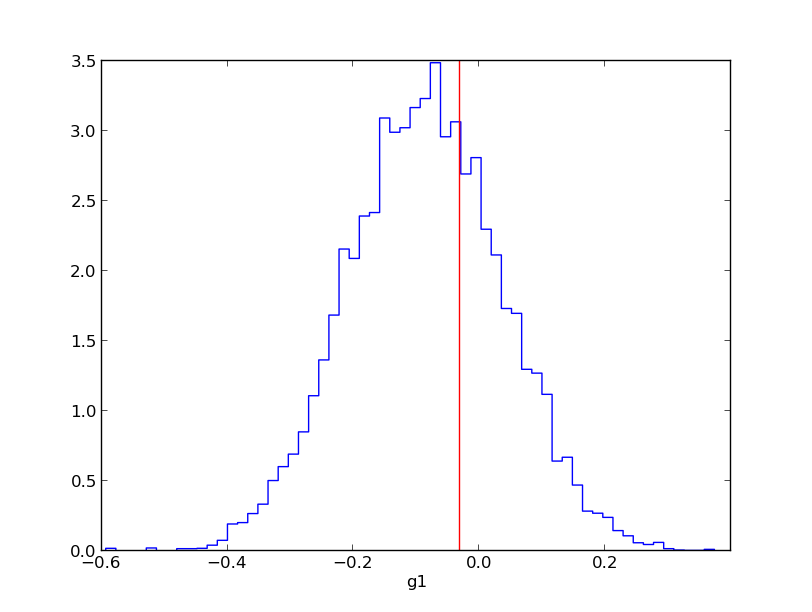
\includegraphics[scale=0.48]{fig/g1hist}

\caption{The figure shows the histogram of posterior samples of g1 in a random patch. The vertical line denotes the value of true(input) g1. }
\end{figure}

\subsection{Bias Test}
In principle given the correct intrinsic shape distribution, the Bayesian inference method would have no bias, if propagate the whole likelihood function.
However, in practical, the bias may be introduced by the model we use for the intrinsic shape distribution,
and the prior regularizer of the prefactor $\xi$ as well as the Gaussian approximation we did for the likelihood
function of $\vec{g}$. Therefore a bias test is necessary to identify how much bias there is. 
Following Heymans et al. (2006), we quantify the systematic bias 
in terms of the multiplicative error m and additive error c on the
true shear $g^{true}$ 
\begin{equation}
\hat{g_{i}}-g_{i}^{true}=m_{i}g_{i}^{true}+c_{i}
\end{equation}

To isolate out the source of the bias in this section, we assume we have perfect measurement on galaxy shape.
We will discuss more on the influence of measurement error section 3.4 .

We calculated the value of $\hat{g}-g^{true}$ of 10,000 data. Each data set has 64 patches and 8$\times$64 galaxies, and
the true(input) P($\epsilon_{0}$) is Beta(2.8,2.8) distribution. The step function model is used with the prior prefator $\xi=3$.
The input true values of $\vec{g}_{1}$ and $\vec{g}_{2}$ of the 64$\times$10,000 sky patches are generated randomly from a uniform distribution from -0.1 to 0.1 . 

As described in section 3.1, we use the mean of posterior samples as the most probable $g_{i}$ and 
the standard deviation as uncertainty. A weighted minimum $\chi^{2}$ linear fit is performed to get the
most-likely value and uncertainty of m and c.
 
Due to the limitation of galaxy number we are not able to get an exact value for m and c. However in our result 
both the most-like and uncertainty of m are around $10^{-3}$ and for c they are around $10^{-4}$ . Due to the
relatively large uncertainty, it is only an rough estimate of bias level.
\begin{figure}
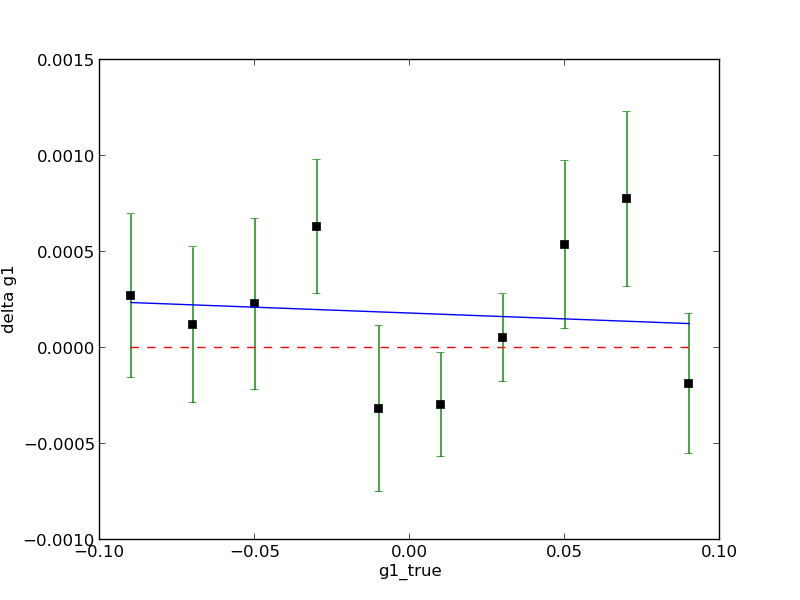
\includegraphics[scale=0.5]{fig/g1bias}

\caption{The figure shows the estimated $g_{1}$ values minus the true (input)
$g_{1}^{true}$. The distribution range of $g_{1}^{true}$ is from
-0.1 to 0.1. Originally there are 640,000 true $g_{1}$. We bin the
plot for presentation purpose. The data point and error bars are the weighted
 average and  variance of $\delta g_{1}$ in each bin. The blue
line is the result of weighted linear fit of the original 640,000 data points
with sample standard deviation as error bar.}
\end{figure}
Suppose we have perfect measurements on galaxy shape. The measured ellipticity then equals to the true lensed ellipticity. With equation (1) the mean ellipticity
estimator has following expression :
\begin{equation}
<\epsilon_{\ell}>=g^{t}+<\epsilon_{0}>+<(\epsilon_{0}+g^{t})[-g^{t*}\epsilon_{0}+O(g^{t*}\epsilon_{0})]>
\end{equation}
When the unlensd ellipticity is isotropic ,we have $<\epsilon_{\ell}>=g^{t}$ . In this case, the mean ellipticity estimator is 
unbiased.
Meanwhile we find that simply using the posterior mean as the estimator of $g$ will lead to a significant bias. 
Figure 3 shows the result of bias test for both mean ellipticity and posterior mean estimator.

\begin{figure}

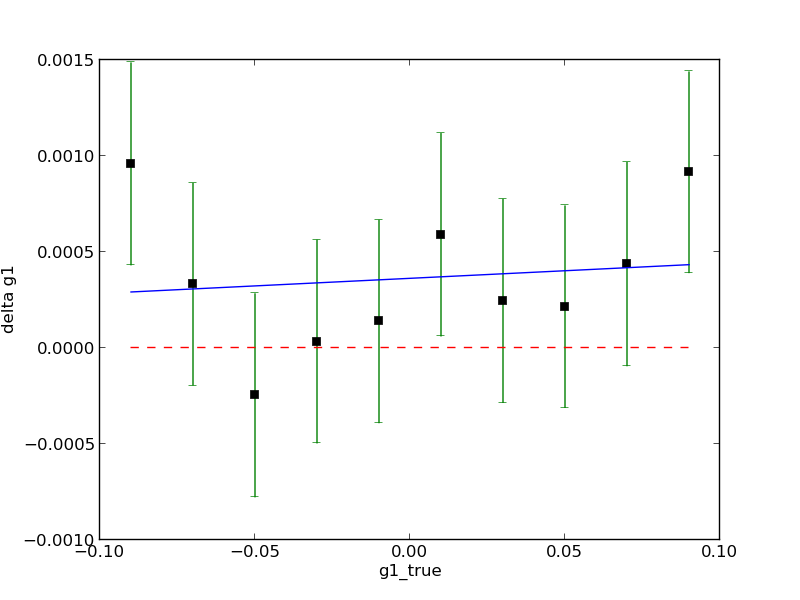
\includegraphics[scale=0.48]{fig/averagebias}

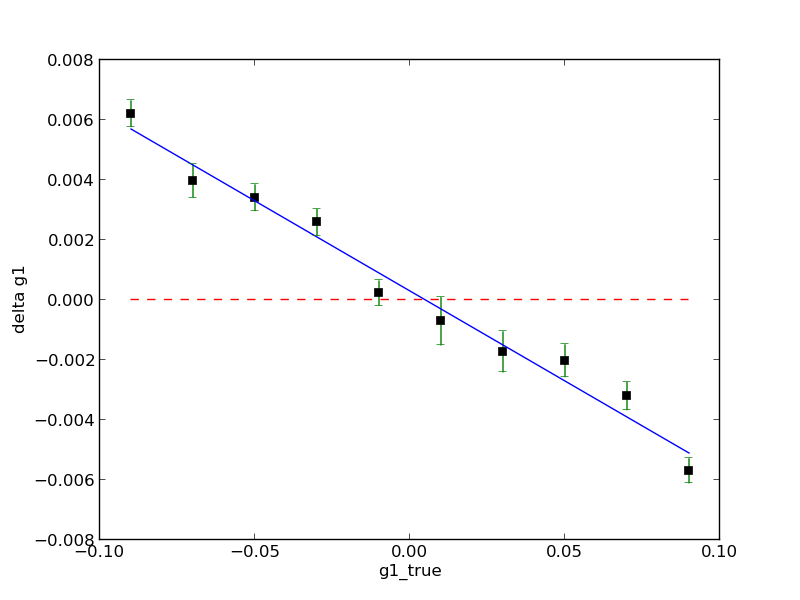
\includegraphics[scale=0.48]{fig/bayesianbias}

\caption{The upper panel shows the systematic bias of the mean ellipticity
estimator. m=$7.9\times10^{-4}\pm0.0029$ , c=$3.63\times10^{-4}\pm1.637\times10^{-4}$.The
lowwer panel shows the systembatic bias of the sample mean. m=$-0.06\pm0.00253$,
c=$3\times10^{-4}\pm1.55\times10^{-4}$ . For both cases the m,c values
are obtained from unweighted linear fit using 640,000 data points. We bin the plot into ten bins for presentation
purpose. The black square denotes the mean of $\Delta g$ in that
bin.}
\end{figure}

\subsection{Accuracy Test}

In this section we calculate the mean square error of mean of posterior samples from the true(input) $g$.  We show that the mean of posterior samples has smaller mean square error than the mean ellipticity estimator but has higher mean square error than the direct Bayesian estimates which could be made if we knew the exact intrinsic shape distribution.
In figure 5 we show how the mean square error changes with the number of galaxies and patches, and make a comparison with mean ellipticity estimator and direct Bayesian estimates. From the figure we can see that when the number of sky patches is small our hierarchical Bayesian method does not necessarily has lower mean square error than mean ellipticity estimator. However it becomes smaller and approach to the result of direct Bayesian estimate which is the best estimate we can possibly make.


\begin{figure}
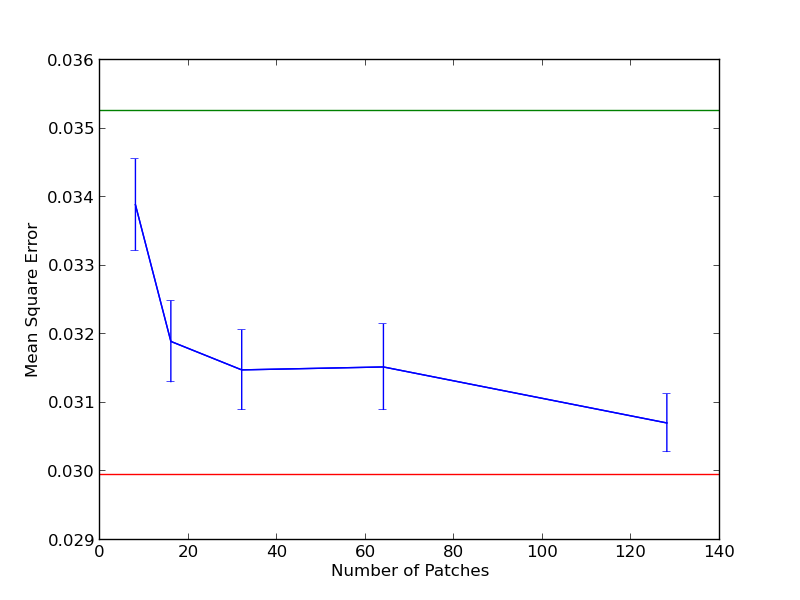
\includegraphics[scale=0.48]{fig/Np_step}

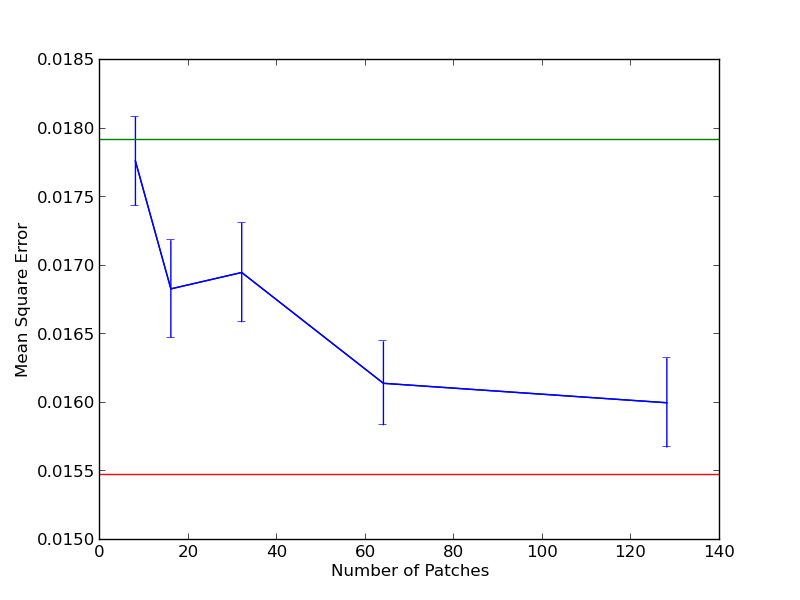
\includegraphics[scale=0.48]{fig/N16NP_vary}

\caption{The upper panel shows how the mean square error of g estimates varies
with the number of patches used with 8 galaxies in each patch. The
lowwer panel shows the same thing with 16 galaxies in each patch. The green line in both graphics shows the mean square error of mean ellipticity estimator,while the red line is the mean square error of g estimates from the likelihood built with the true intrinsic shape distribution. They are both independ from the number of patches. }
\end{figure}


\subsection{Measurement Error}
In this section we  discuss how the shape measurement error 
affects the variance and bias of shear inference.
In principle, if the likelihood of true lensed ellipticity $p(\epsilon_{ob}|\epsilon_{\ell})$
is known the likelihood $p(\epsilon_{ob}|g,\alpha)$ can be calculated using the convolution as equation (7).
However, due to the limitation of computational time we avoid to do this convolution but use $\epsilon_{ob}$
as an estimator of $\epsilon_{\ell}$.
The likelihood of true lensed ellipticity $p(\epsilon_{ob}|\epsilon_{\ell})$ we use in the simulation is a 2D
Gaussian with mean equals $\epsilon_{\ell}$ and $\sigma$ equals 0.05 .
Figure 5 shows the mean square error of the sample mean estimates in comparison with mean ellipticity estimator.
\begin{figure}
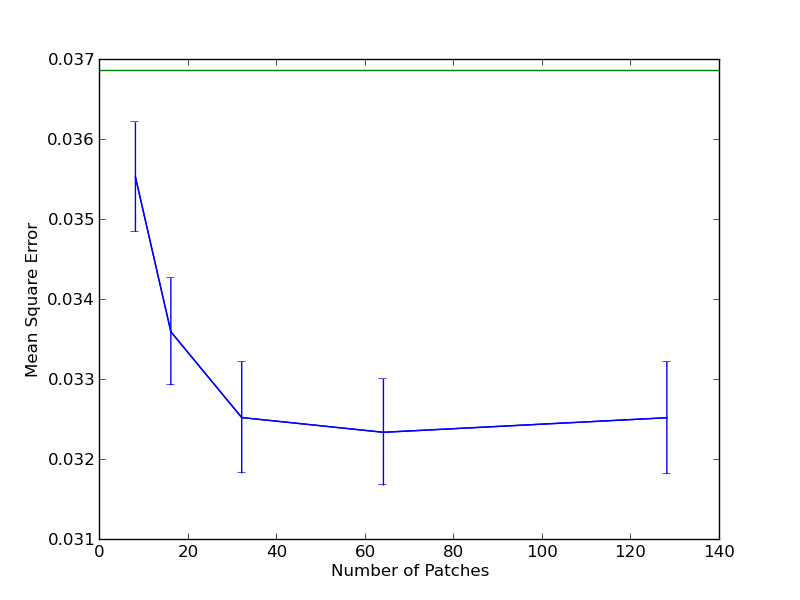
\includegraphics[scale=0.48]{fig/errorN8}
\caption{Figure 5 shows how the mean square error of sample mean estimate varies with the number of patches used, while shape measurement error is considered as described in Section 3.4 .
The horizontal line denotes the mean square of mean ellipticity estiimator which does not depend on number of patches. }
\end{figure}



\subsection{Prefactor $\xi$}

One limitation of the step function model is that it needs to be \textit{regularized};
this is achieved by assigning a prior PDF for the step heights $\vec{\alpha}$.
We use the form $Prior(\vec{\alpha}|\xi)=exp(-\xi\sum(\alpha_{i}-\alpha_{i-1})^{2})$
when inferring the P($\epsilon$) and $g$. The choice of this functional
form corresponds to the assumption that the true P($\epsilon$) is
smooth, which seems fairly natural. This function has a hyperparameter,
$\xi$, that needs to be set somehow. If $\xi$ is too small, the
inferred P($\epsilon$) will be too noisy, and the accuracy of the
$g$ inference will decrease. Likewise, choosing an $\xi$ that is
too large, the inferred P($\epsilon$) will be too smooth, and the
data will be under-fitted. In principle one could infer $\xi$ form
the data at hand, but in practice we find that we further more need some
prior regularizer on $\xi$ to obtain correct inference. Therefore in this paper 
we just tuned $\xi$ empirically. From various trials, We find
that $\xi$ should be proportional to the mean data number density and can
be approximated by the following empirical formula: 
\begin{equation}
\xi=N<\rho(|\epsilon|)>/256*\frac{Nbin}{10}
\end{equation}
Here $<\rho|\epsilon|>=\int\rho(|\epsilon|)^{2}d(|\epsilon|)$ corresponds
to the average of data number density, and Nbin is the number of bins used 
in step function model. 

%%%%%%%%%%%%%%%%%%%%%%%%%%%%%%%%%%%%%%%%%%%%%%%%%%%%%%%%%%%%%%%%%%%%%%%%
%%  SECTION N: XXX
%%%%%%%%%%%%%%%%%%%%%%%%%%%%%%%%%%%%%%%%%%%%%%%%%%%%%%%%%%%%%%%%%%%%%%%%



\section{Discussion}

\label{sec:XXX} In weak lensing survey, one way to obtain high S/N
ratio is to stack large number of lensing signal together, and calculate
the mean shear map of all these lensing systems. However simply 
stacking all the lensing signals would not be the optimal way because
the amount of information we can obtain from each lensing system
can be very different. The Bayesian inference approach we proposed
allows a natural way to optimally include all the data. Instead of
stacking what we need to do is to propogate the likelihood of the
shear map of each lensing system. The statistical property of all
the lensing systems like the galaxy-mass, shear-shar correlation function
, in principle can be calculated from these likelihood functions.

Several  model fitting  shape measurent methods have been proposed in recent years.
Unlike the average method which merely request a point estimator of galaxy ellipcity, our 
hierachical bayesian approach utilizes the whole likelihood of the galaxy ellipticity in a Bayesian probability analysis framework.


%%%%%%%%%%%%%%%%%%%%%%%%%%%%%%%%%%%%%%%%%%%%%%%%%%%%%%%%%%%%%%%%%%%%%%%%
%%  SECTION X: CONCLUSIONS
%%%%%%%%%%%%%%%%%%%%%%%%%%%%%%%%%%%%%%%%%%%%%%%%%%%%%%%%%%%%%%%%%%%%%%%%



\section{Conclusions}

\label{sec:conclusions}

In summary, we have presented a conceptually hierachical inference
approach for weak lensing shear estimation, with carefully calculated 
uncertainty estimates. This method is intrinsically cope with high noise
levels on the input data and naturally allows bad fit to be identified 
from the residuals map. We also have proposed a flexible non-parametric model 
for intrinsic shape distribution allows us to obtain the correct posterior 
distributions, while avoiding making any unsupported assumptions. The Gibbs
sampler allows us to sample the posterior distribution of shear in large number of
sky patches simultaneously and efficiently.


\begin{itemize}
\item We ...
\item The ...
\item The ...
\end{itemize}
%%%%%%%%%%%%%%%%%%%%%%%%%%%%%%%%%%%%%%%%%%%%%%%%%%%%%%%%%%%%%%%%%%%%%%%%
%%  ACKNOWLEDGMENTS
%%%%%%%%%%%%%%%%%%%%%%%%%%%%%%%%%%%%%%%%%%%%%%%%%%%%%%%%%%%%%%%%%%%%%%%%



\section*{Acknowledgments}

We thank XXX for useful discussions and suggestions.

YT acknowledges ....
%
DWH acknowledges support from ...
% 
PJM was given support by the Royal 
Society in the form of a research fellowship.
%
% Code used? Links to repositories?


%%%%%%%%%%%%%%%%%%%%%%%%%%%%%%%%%%%%%%%%%%%%%%%%%%%%%%%%%%%%%%%%%%%%%%%%
%%  APPENDICES
% %%%%%%%%%%%%%%%%%%%%%%%%%%%%%%%%%%%%%%%%%%%%%%%%%%%%%%%%%%%%%%%%%%%%%%
% 
% \appendix
% 
% \section{}
% \label{sec:appendix}
% 
% 
%%%%%%%%%%%%%%%%%%%%%%%%%%%%%%%%%%%%%%%%%%%%%%%%%%%%%%%%%%%%%%%%%%%%%%%%
%%  REFERENCES
%%%%%%%%%%%%%%%%%%%%%%%%%%%%%%%%%%%%%%%%%%%%%%%%%%%%%%%%%%%%%%%%%%%%%%%%


% MNRAS does not use bibtex, input .bbl file instead. 
% Generate this in the makefile using bubble script in scriptutils:


%   bubble -f PS1QLS-survey.tex references.bib 


 \bibliographystyle{apj}
\bibliography{references}
 %\input{PS1QLS-survey.bbl}


%%%%%%%%%%%%%%%%%%%%%%%%%%%%%%%%%%%%%%%%%%%%%%%%%%%%%%%%%%%%%%%%%%%%%%%%


\label{lastpage} \bsp

\end{document}

%%%%%%%%%%%%%%%%%%%%%%%%%%%%%%%%%%%%%%%%%%%%%%%%%%%%%%%%%%%%%%%%%%%%%%%%

\end{document}
